%De l'importance et de la place de la communication externe dans l'associatif
%TODO remplacer le titre par celui de la fiche contrat pédagogique.

\section {Introduction}

    Depuis bientôt 4 ans, je suis mes études à l'Insa.
    La première chose que l'on m'as dite sur cette école, avant même son nom, ce fût l'importance de la composante humaine de la formation par rapport à d'autres établissements. Ce travail en est d'ailleurs la preuve.

    Depuis bientôt 4 ans, j'ai eu l'occasion de travailler dans plusieurs associations : le Ski Club, l'AEDI, le BDE, les 24h pour ne citer que les plus importantes.
    Toutes ces expériences ont en commun ma passion pour les arts graphiques et la communication visuelle.

        
    
\section{But de la communication extérieure}

    Le but premier de la communication est de promouvoir les services, ou actions de l'association.
    Dans le cas du ski club, ce sera les sorties proposé et la location, pour les 24h, ce sera la festival, et autres soirées, pour le bde, ce sera les services et évènement organisé.
    Mais on peut prendre aussi l'exemple du forum Rhône Alpe, de la plupart des association de département etc ...

    Tout le travail effectué en communication extérieur, est principalement tournée vers la promotion des autres actions faites par l'association.
    Un seul contre exemple me viens en tête, il s'agit des cartes de vœux envoyé par les 24h au partenaires.
    Mais, en un sens, il peut également s'agir de promotion, puisque ça contribue à garder de bonne relation, et à pérenniser les partenariats commerciaux.


\section{Mes expériences dans l'associatif}

    \subsection{Le ski club}
        
        Depuis tout petit, j'ai l'habitude de faire du ski à chaque hiver. Pour garder cette habitude, je me suis inscrit dès ma première année comme membre actif du Ski club.
        
        L'ancien webmaster quittait l'Insa l'année de mon arrivé, je me suis donc proposé de reprendre le site de l'association pour le maintenir.
        Ce fut ma première expérience relative à la communication dans l'associatif.
        J'ai entièrement reconstruit le site web, pour améliorer la visibilité en ligne de l'association.
        
        Le site comportait des informations concernant l'organisation des sorties, du weekend, ainsi que sur la location ou l'entretien de matériel.
        
        Je ne fais plus parti du skiclub, le site à donc été remplacé par les membres actifs.
        
    \subsection{L'AEDI}
        
        Il serait faux de dire que je suis membre de l'AEDI. Je n'ai fais que proposer mon aider en cas de besoin.
        Mais j'ai eu l'occasion de dessiner un visuel de T-Shirt distribué aux "bizuth" lors du weekend d'intégration, et différentes affiches pour le barbecue de fin d'année.
        Ces travaux étaient d'une durée très courte, cela ne m'a pas empêché néanmoins d'en tirer de bonnes expériences.
        
    \subsection{Les 24 heures de l'Insa}
        
        Cela fait 2 ans que je suis dans l'équipe communication des 24h de l'insa, et c'est probablement pour cette association que j'ai fourni le plus de travail.
        Les 2 années j'ai dessiné un certain nombre de ressources qui ont été réutilisé sur différents supports, tels que les programmes, les gobelets, les T-Shirts, les affiches etc ...
        J'ai également participé, entre autres, à l'élaboration des affiches journées et concerts.
        
        J'en tire de bonne expériences notamment en ce qui concerne la suivi d'un projet sur une plus longue durée.
        
    \subsection{Le BDE}
    
        J'ai également travaillé sur plusieurs projets avec l'équipe communication du bde.
        Cependant, ayant intégré l'équipe en cours d'année, je n'ai pas eu l'occasion de faire des travaux très significatifs.

\section{Observations}

    La première observation que j'ai pu faire aussi bien au sein de l'équipe com du BdE que des 24h, est que la communication externe n'est pas toujours à la hauteur pour promouvoir les efforts fourni par les autres services.
    Soit à cause d'un retard, d'un manque de moyen, ou d'un manque d'efficacité.

    \subsection{BdE}

        Par exemple, au BdE, comparativement à la médiatisation que l'on peut voir dans la plupart des entreprises, le bde a un service de communication sous-estimé et qui, je pense, devrait être plus important afin de mieux faire connaitre les services proposé aux étudiants. Je sais très bien que ce n'est pas comparable. La survie d'une entreprise dépend souvent en grande partie de sa visibilité. Malgré tout, %TODO Continuer
    
    \subsection{24 heures de l'Insa}
        
        En revanche, la communication au 24h est plus importante et mieux planifié, parce qu'indispensable à la manifestation, mais elle n'est souvent pas assez organisé pour avoir des ressources vraiment utilisable d'une année sur l'autre.
        Bien qu'un effort soit fait de ce côté là, et, pour donner un exemple, les photos prises sur la manifestation d'une année sur l'autre sont souvent réutilisé dans plusieurs support de communication, tels que le site web, ou les plaquettes destinées aux sponsors.
        
    Cependant, on peut nuancer cette remarque, en notant que d'une part, les services du BdE ne pâtissent pas de cette mauvaise visibilité, et sont toujours d'une grande aide aux étudiants. D'autre part, les 24h bénéficient déjà d'une grande notoriété auprès d'un certains publics, et une campagne de communication faites au dernier moment ne nuiras pas au festival, ni à son image. Le but est plus d'informer que d'attirer de nouveaux publics.
    %TODO remanier faites au dernier moment.
    
\section{Déboires : pièges à éviter}

    Je vais revenir sur plusieurs gros projets, en analysant quels étaient les difficultés, les enjeux, et pourquoi ces projets n'ont pas aboutie, ou mal aboutie.
    
    \subsection{La bache de la MdE}
    
        Le bde ayant de fort partenariat avec Perstil, ceux-ci nous proposèrent une impression gratuite sur une bâche de 8m par 1m, avec pour celle contrainte, un bandeau publicitaire au bas.
        La décision fut prise de placer cette bâche au devant de la MdE, sur la rambarde du balcon, pour attirer un peu plus l'œil et signaler la présence de la MdE.
        Quand je suis arrivé dans l'équipe, cette proposition était déjà lancé depuis quelques année, mais personne ne s'était mis à la tâche.
        Je me suis donc proposé de travailler dessus pendant l'été. Et après quelques réunions, le thème choisi serait "Urbano-floral".
        
        L'erreur que je peux relever ici, c'est qu'on entame un travail aussi important, 2 mots ne peuvent vraiment pas définir un thème.
        
        Je suis donc parti avec des idées en tête. Et chacun fit de même en interprétant le thème différemment.
        Pour la plupart des ébauches que je présentait, les membres de l'équipe étaient en désaccord, et le projet fini par stagné puisque plus rien n'était approuvé.
        
        Je pense donc qu'il aurait fallu pour ce travail, ne pas s'arrêter à deux mots, mais réellement se mettre d'accord sur un style visuel, et sur les attentes du résultat.
        Pourquoi faire ce travail, qu'est ce qu'on attendra du résultats, dans quel registre peut-on se placer ?
        %TODO à réécrire.
        
    \subsection{Les affiches Journées et Concerts des 24h}
        
        Un des travail les plus important pour l'équipe communication des 24h, est la réalisation des affiches Journées et Concerts.
        Ce sont deux affiches imprimé au format B1, en grand nombre et qui sont en grande partie responsable de la visibilité des 24h sur Villeurbanne et Lyon.
        
        Chaque année, des proposition de thème et des ébauches d'affiches sont présentés plusieurs mois avant la manifestation, afin que l'équipe entière des 24h puisse juger et voter pour un thème.
        L'an dernier, les deux idées qui s'étaient démarqué étaient une reprise des lapins suicidaires de Andy Riley, et un thème dont la ligne directrice était l'aspect BD.
        Nous avons alors choisis d'utiliser les 2 thèmes.
        %TODO inutile de détailler autant.
        J'avais une idée très précise de ce que je pensais faire, et elle semblait plaire à l'équipe.
        
        Entre temps, l'idée des lapins suicidaires à été abandonné, pour des raison évidentes.
        Nous avons donc remplacer dans la précipitation les lapins par des pandas.
        
        J'ai commencé à proposer des ébauches, et le travail avançait bien.
        Cependant, au fur et à mesure que j'avançais, de plus en plus de remarques m'ont été faites. Tels détails serait mieux ainsi, ou tel autres autrement, etc ...
        Au fur et à mesure que le travail avançait, le nombre de remarque augmentait, et plus j'approchais du résultat finale, plus il semblait déplaire.
        C'est comme ça, que quelques jours avant l'envoi pour impression, il à été décidé de recommencer presque de zéro pour produire une affiche différente et exempte de toutes les remarques faites à la précédente.
        
        De mon avis, c'était un travail bâclé, bien plus critiquable que la précédente affiche, mais sous prétexte de la précipitation, l'avis générale à été, "nous n'avons plus le temps de faire des remarques, il faut agir".
        
        Je pense que bien qu'il faut prendre en compte les remarques faites, il faut surtout prendre du recul, et éviter de les suivre automatiquement. C'est comme ça que l'on perd la cohésion de son idée, et que le travail final perd de son intégrité.
        
        Pour exemple, je me suis penché sur la façon de procéder du festival Rock'n'Solex, qui est très proche des 24h de l'Insa (festival étudiant organisé par l'Insa de Renne).
        Ils ne travaillent pas eux même sur l'affiche, mais lancent un concours. Ils ont une réputation suffisante pour que les travaux proposé soient d'une certaine qualité.
        Quelques modification sont faites sur l'affiche gagnante, puis c'est l'impression.
        
        La grande différence, c'est qu'ils choisissent parmi des travaux déjà aboutie, et complet, qui ont déjà un certains caractère et une certaine intégrité.
        
        Je pense donc qu'il faut minimiser le nombre de personne qui peuvent donner leur avis sur les travaux, afin de ne pas se perdre en modifications.
        Et seulement qu'une fois que c'est aboutie, le soumettre au reste de l'équipe. Dans tout les cas, ça ne pourras pas plaire à tout le monde. Mais un travail aboutie est plus facilement acceptable qu'un travail non aboutie, tout simplement parce que ceux qui travail dessus voient déjà la continuité, et l'aboutissement, alors que les autres non.
        %TODO à réécrire.
        
\section{Résultats et conclusion tiré de ces expériences}

    %TODO découper en sous parties

    De manière général, dans l'associatif le travail fourni est important. Je pourrais estimé à 10\% le ratio de travaux qui seront effectivement publié.

    Il y'a effectivement une part du travail qui est dédié à des essais, ou soumis à des sélections ; et également une part du travail qui ne sera jamais aboutie, ou abandonné en cours de route.

    La principale cause de ce gaspillage, est la méthode employé : en effet, il est plus facile de travailler sur une production, de la finir, puis d'en commencer une autre, et ainsi de suite. Ce travail est parallélisé sur plusieurs personnes, pour plus de rapidité.

    %TODO expliquer un peu plus
    Je pense que le plus grand bénéfice que l'on pourrait tiré, c'est de s'obliger à établir une charte graphique claire, pour éviter de s'éparpiller en travaux inutiles.
    Il serais plus judicieux, à mon sens, de travailler sur un ensemble de ressource graphique réutilisable plutôt que de travailler production par production.

    Dans le cas du bde, cette charte graphique est présente, car la communication s'étale tout au long de l'année, et il est indispensable d'avoir une cohérence visuelle.
    En revanche, dans le cas des 24h, du fait que chaque année, le thème change, la production graphique est entièrement à refaire.
    C'est la raison pour laquelle, pendant les 2 ans où j'ai participé à cette équipe, le travail de chacun s'éparpillait dans un nombre incroyable de travaux très intéressant, mais peu voir pas cohérent ensemble, donc inutilisable.

\newpage

\section{Portefolio}

    Je présente ici différents travaux qui illustrent le mieux mon travail, et les évolutions que suis un projet.
    %TODO à remanier.
    \subsection{BdE}
        \begin{center}
            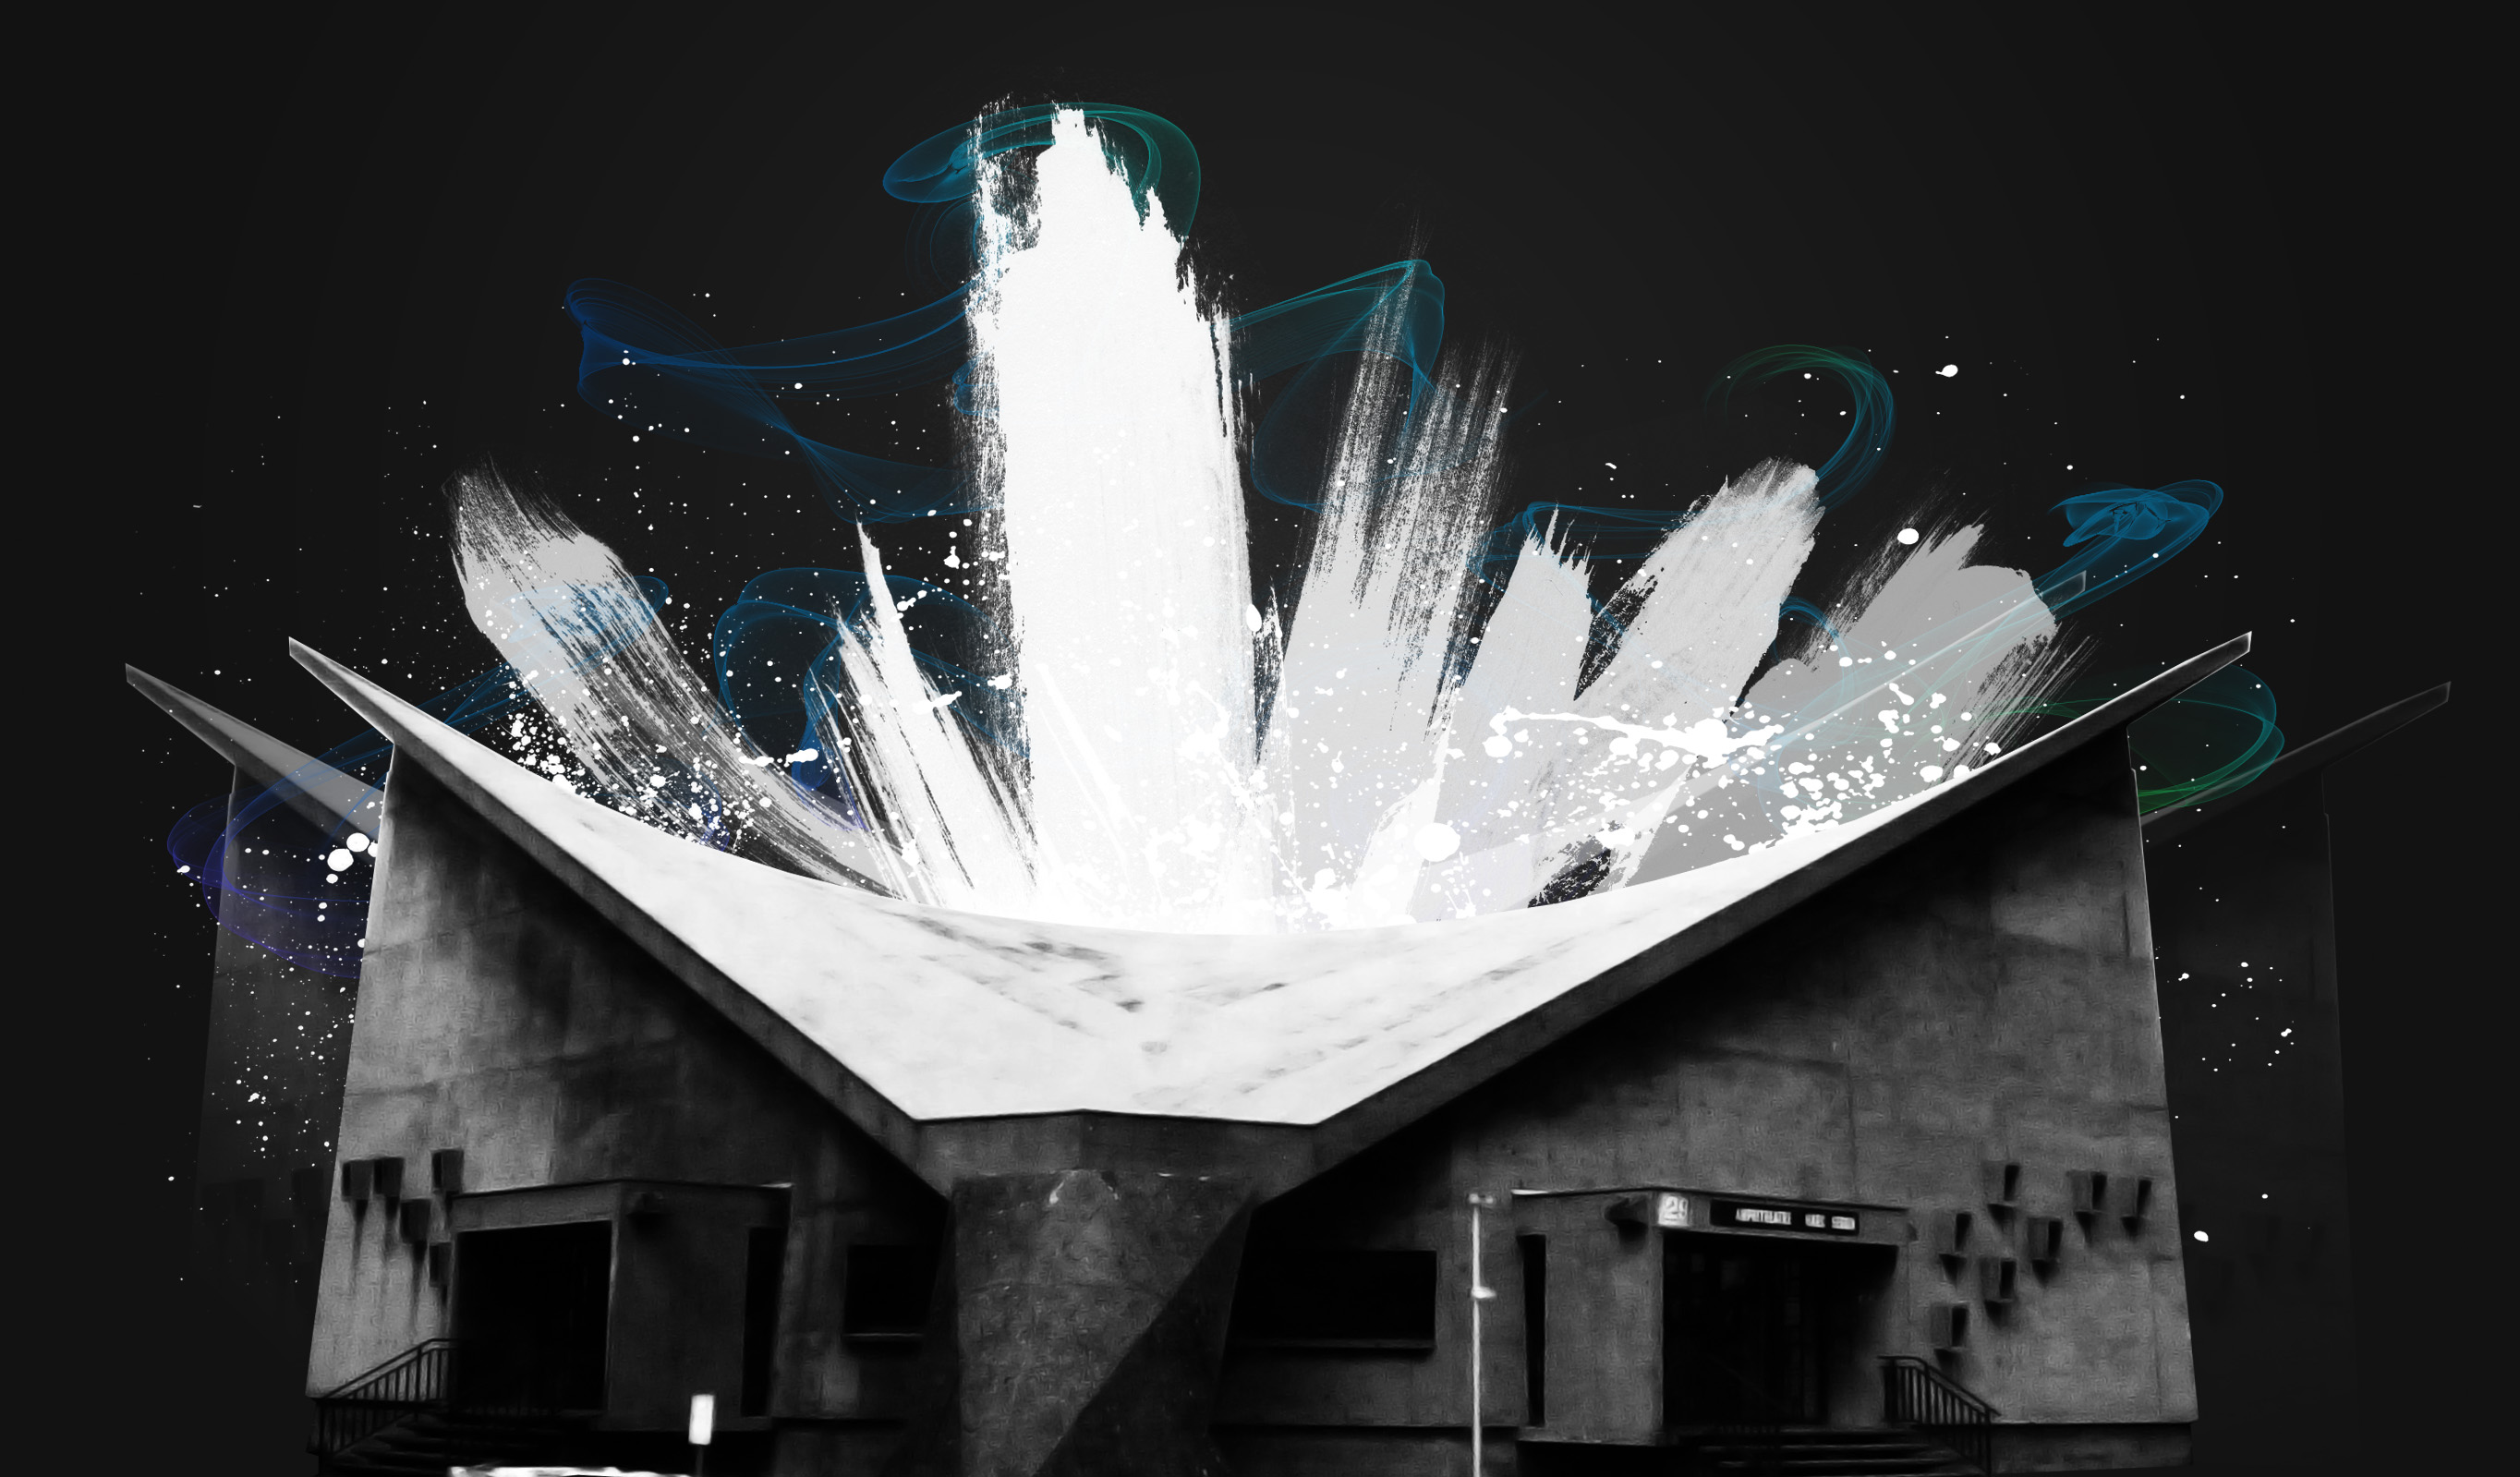
\includegraphics[width=\textwidth]{img/amphi.jpg}\\
            Première esquisse pour la bâche du BdE
        \end{center}

        \begin{center}
            %TODO inclure les autres travaux.
            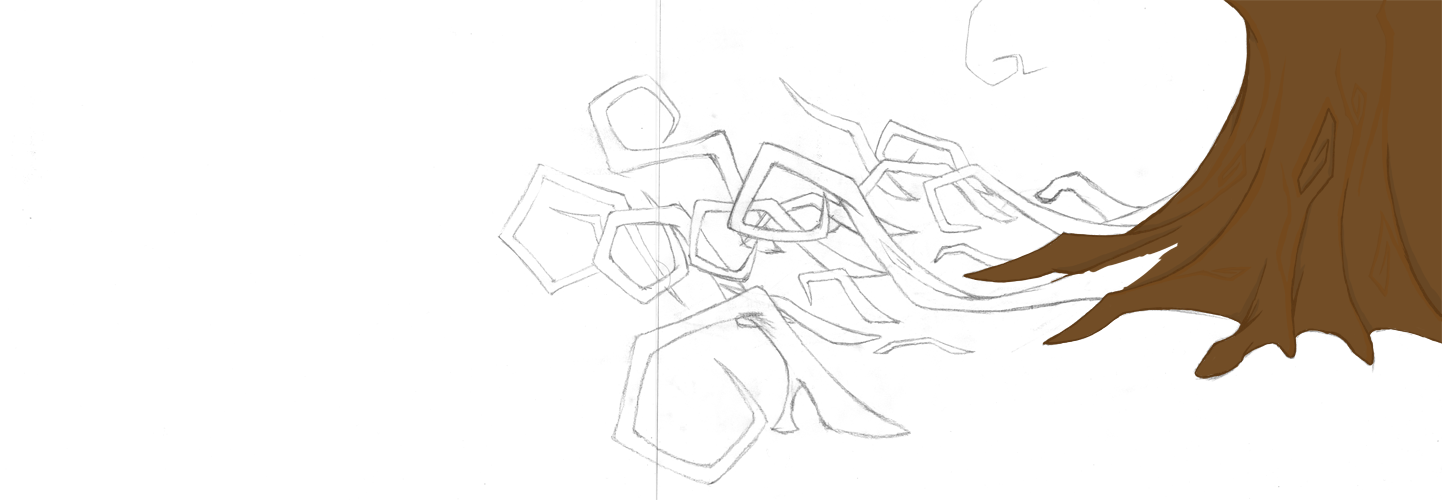
\includegraphics[width=\textwidth]{img/arbre.png}
            
\includegraphics[width=\textwidth]{img/mde.png}
            
\includegraphics[width=\textwidth]{img/mde+arbre.png}
            Différentes ébauche et évolution du travail sur la bâche du BdE.
        \end{center}
            
    \subsection{24h de l'Insa}
    
        \subsubsection{36èeme édition - 2010}
    
            \begin{center}
                \fbox{
\includegraphics[width=0.3\textwidth]{img/preAffiche.png}}
                \fbox{
\includegraphics[width=0.3\textwidth]{img/preAffiche_panda.png}}
                \fbox{
\includegraphics[width=0.3\textwidth]{img/preAffiche_panda_2.png}}\\    
                \fbox{
\includegraphics[width=0.3\textwidth]{img/preAffiche_panda_2leaf_date1.png}}
                \fbox{
\includegraphics[width=0.3\textwidth]{img/preAffiche_panda_2leaf_date2.png}}
                \fbox{
\includegraphics[width=0.3\textwidth]{img/preAffiche_panda_2hot.png}}\\
                \fbox{
\includegraphics[width=0.3\textwidth]{img/preAffiche_panda_3.png}}
                \fbox{
\includegraphics[width=0.3\textwidth]{img/preAffiche_panda_3-2.png}}
                \fbox{
\includegraphics[width=0.3\textwidth]{img/preAffiche_panda_3-3.png}}\\
                Suivi des étapes dans le travail sur l'affiche des 24h de l'insa, 36ème édition - 2010
            \end{center}
            
            \begin{center}
                \fbox{
\includegraphics[width=0.48\textwidth]{img/affiche_concert.png}}
                \fbox{
\includegraphics[width=0.48\textwidth]{img/affiche-concerts-v4-flat2.jpg}}\\
                Affiche proposé et affiche finale  
            \end{center}
            
        \subsubsection{37èeme édition - 2011}            
            
            \begin{center}        
                \fbox{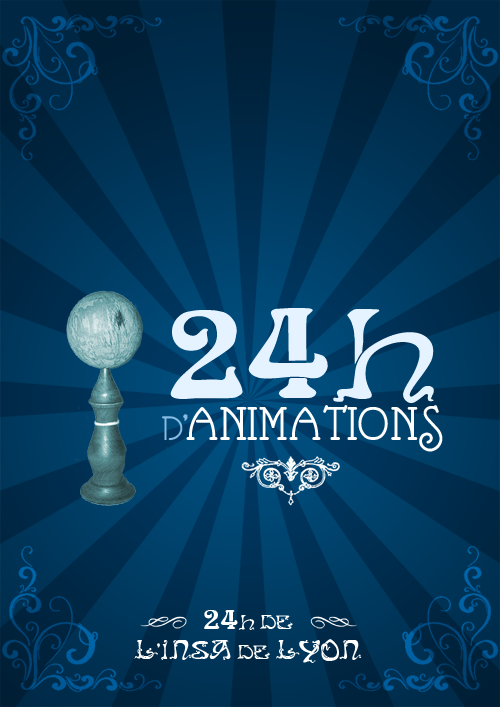
\includegraphics[width=0.3\textwidth]{img/old-preview-animations.png}}
                \fbox{
\includegraphics[width=0.3\textwidth]{img/old-preview-courses.png}}
                \fbox{
\includegraphics[width=0.3\textwidth]{img/old-preview-concert.png}}
                Présentation d'un thème de communication intitulé \emph{Old School}
            \end{center}
            
            \begin{center}           
                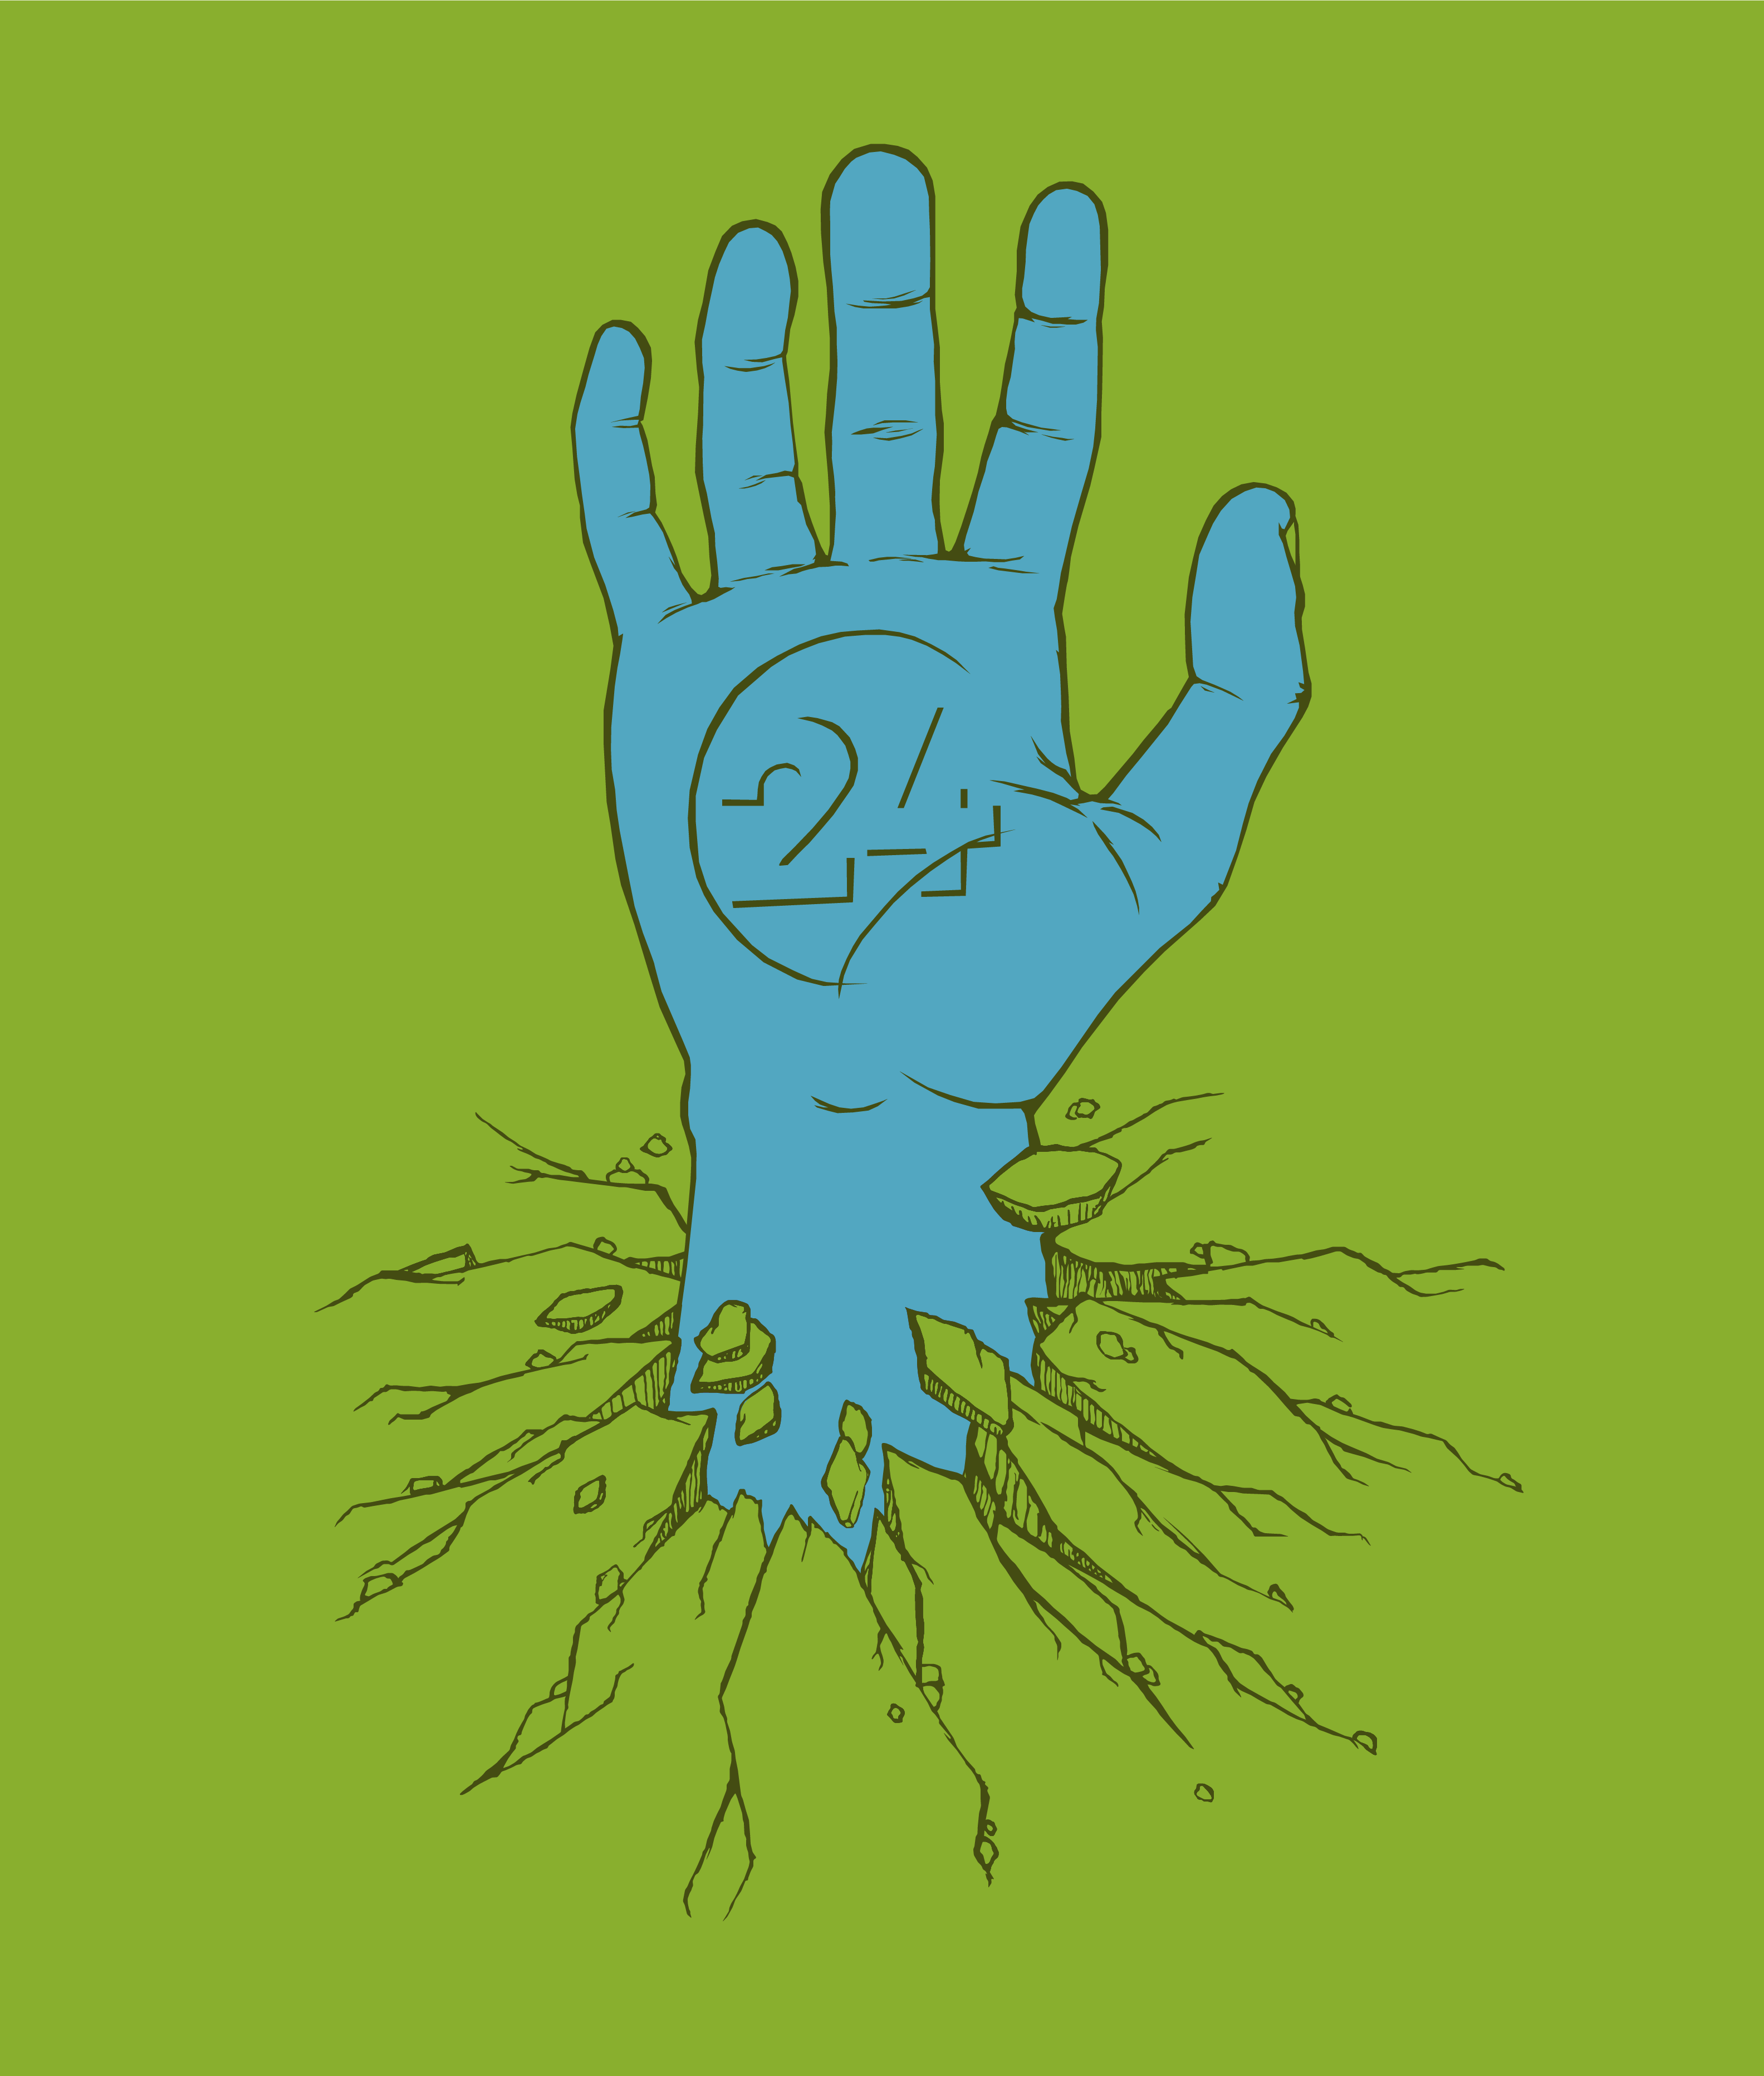
\includegraphics[width=\textwidth]{img/main.png}\\
                ~\\
                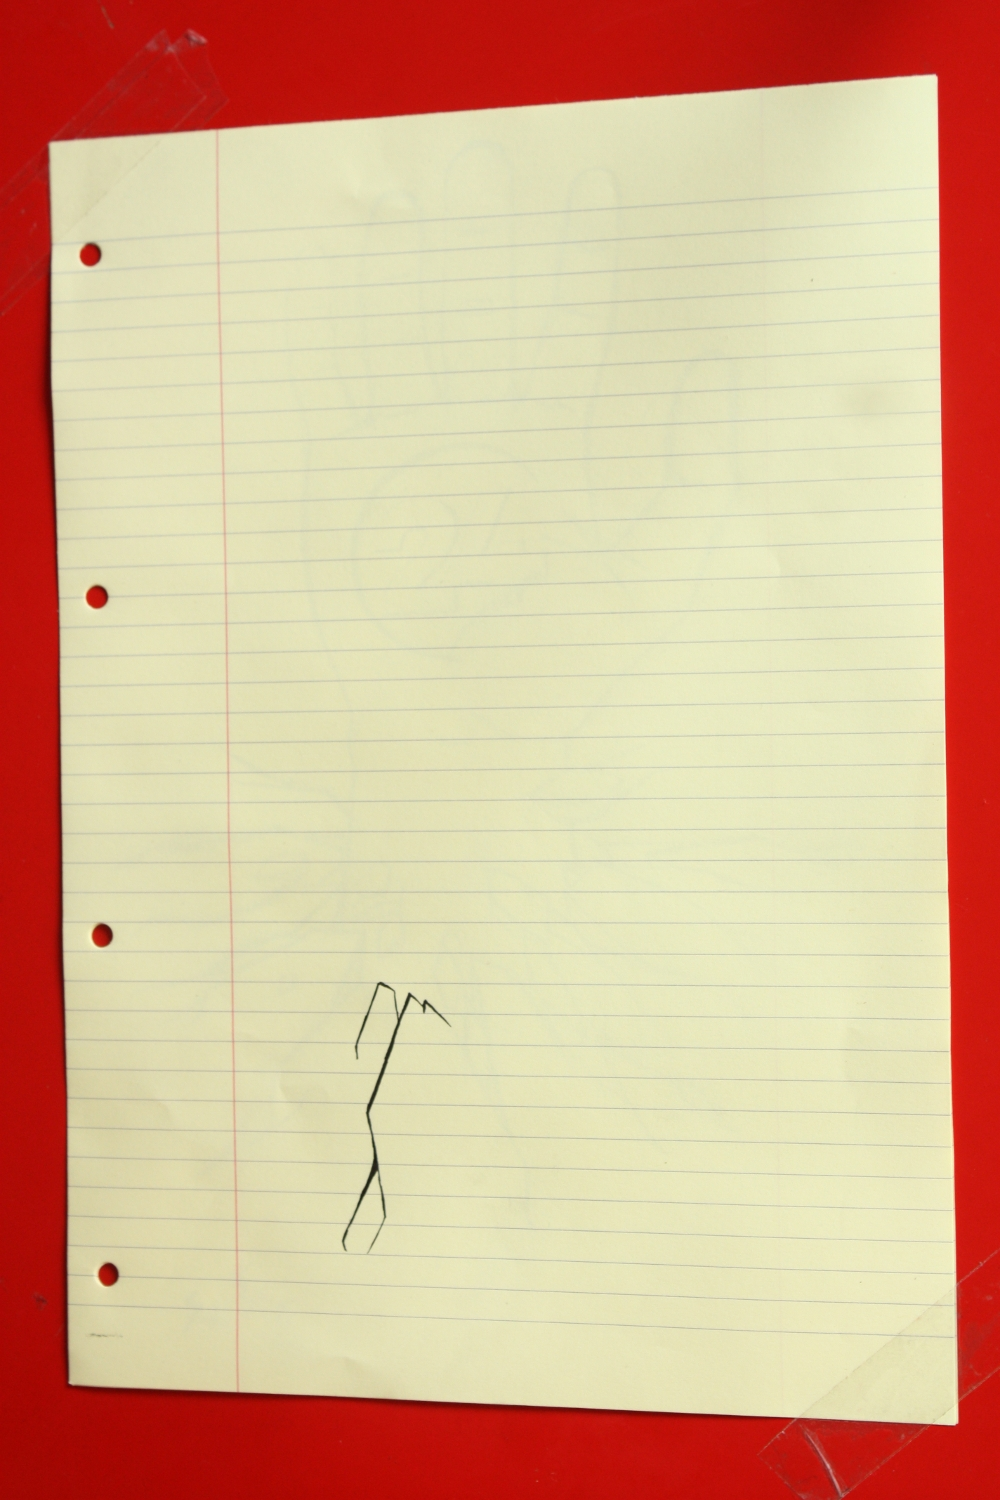
\includegraphics[width=0.24\textwidth]{img/IMG_5730.JPG}
                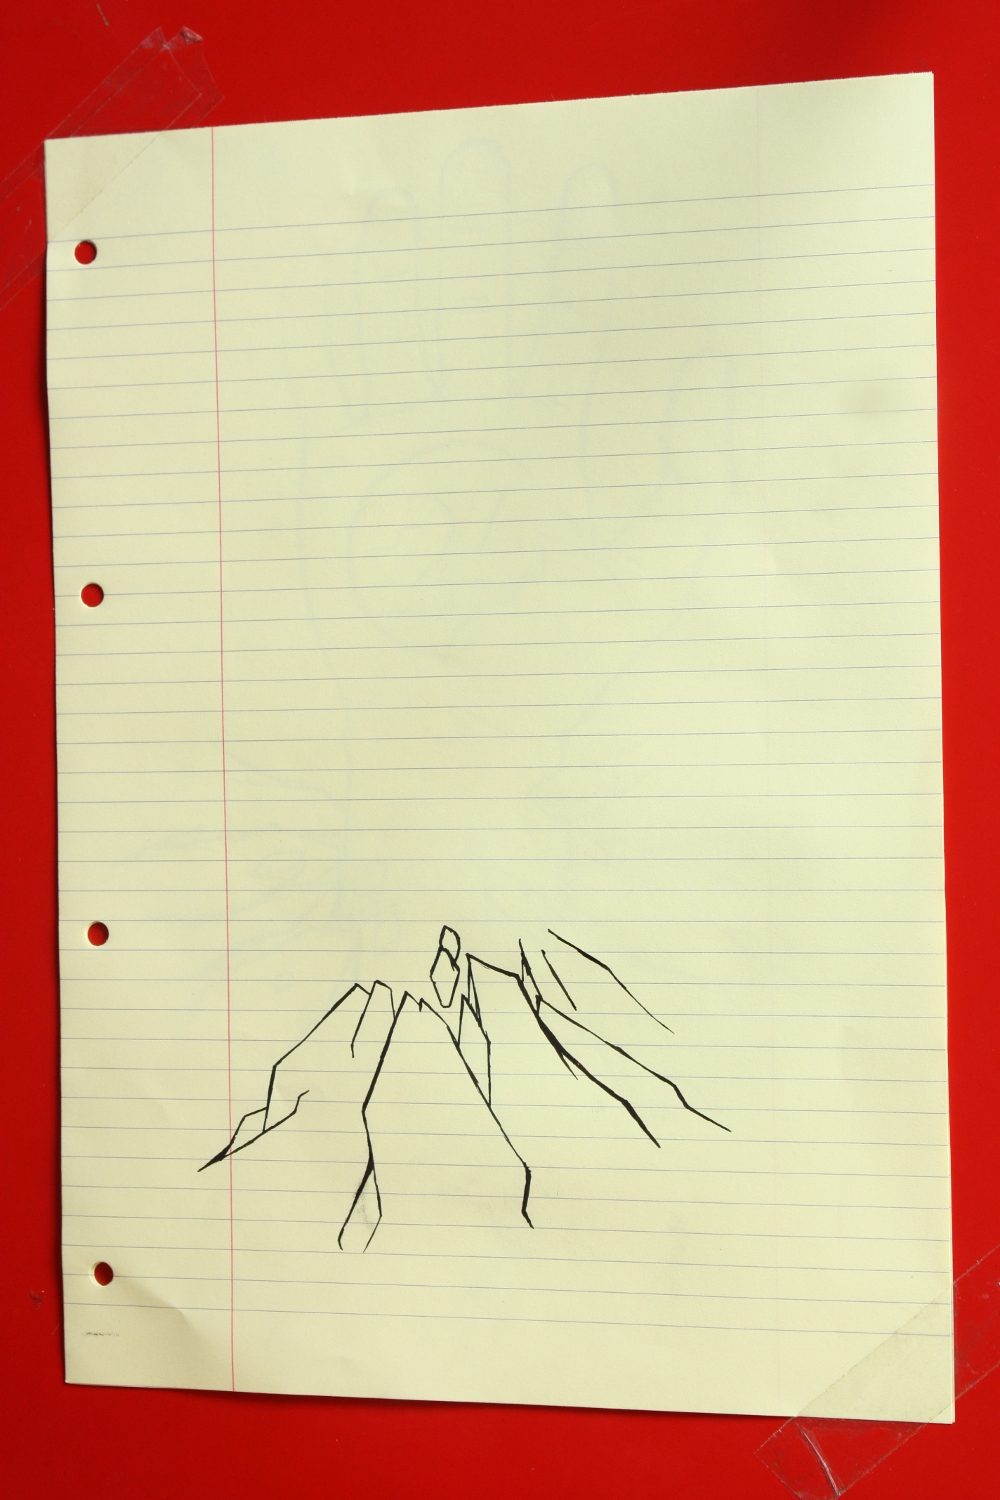
\includegraphics[width=0.24\textwidth]{img/IMG_5741.JPG}
                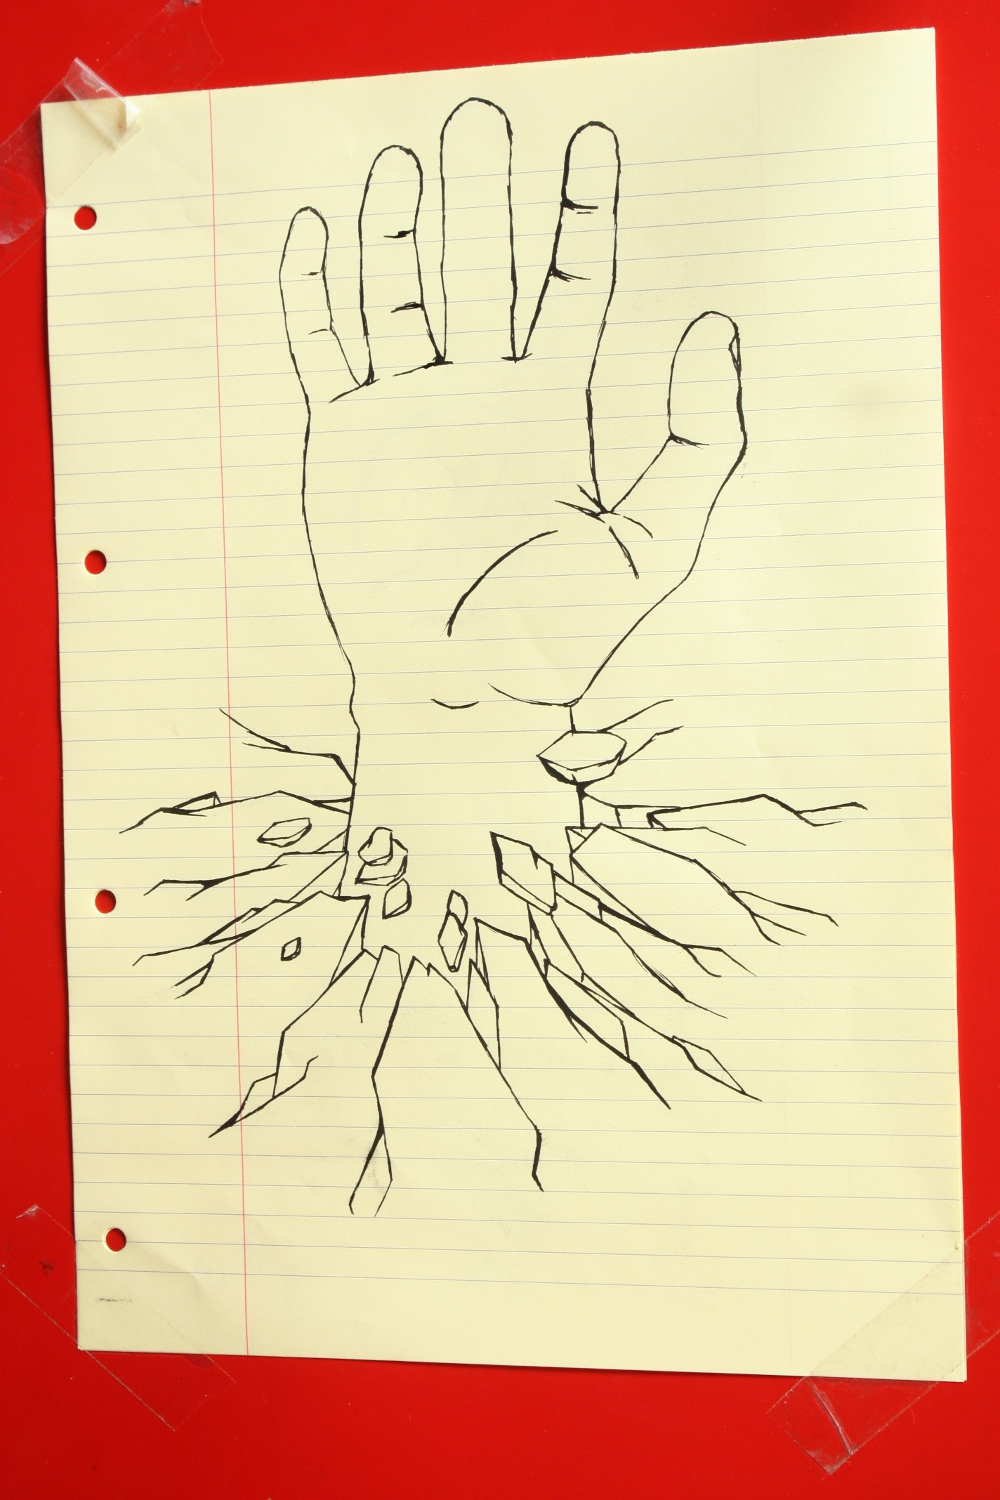
\includegraphics[width=0.24\textwidth]{img/IMG_5792.JPG}
                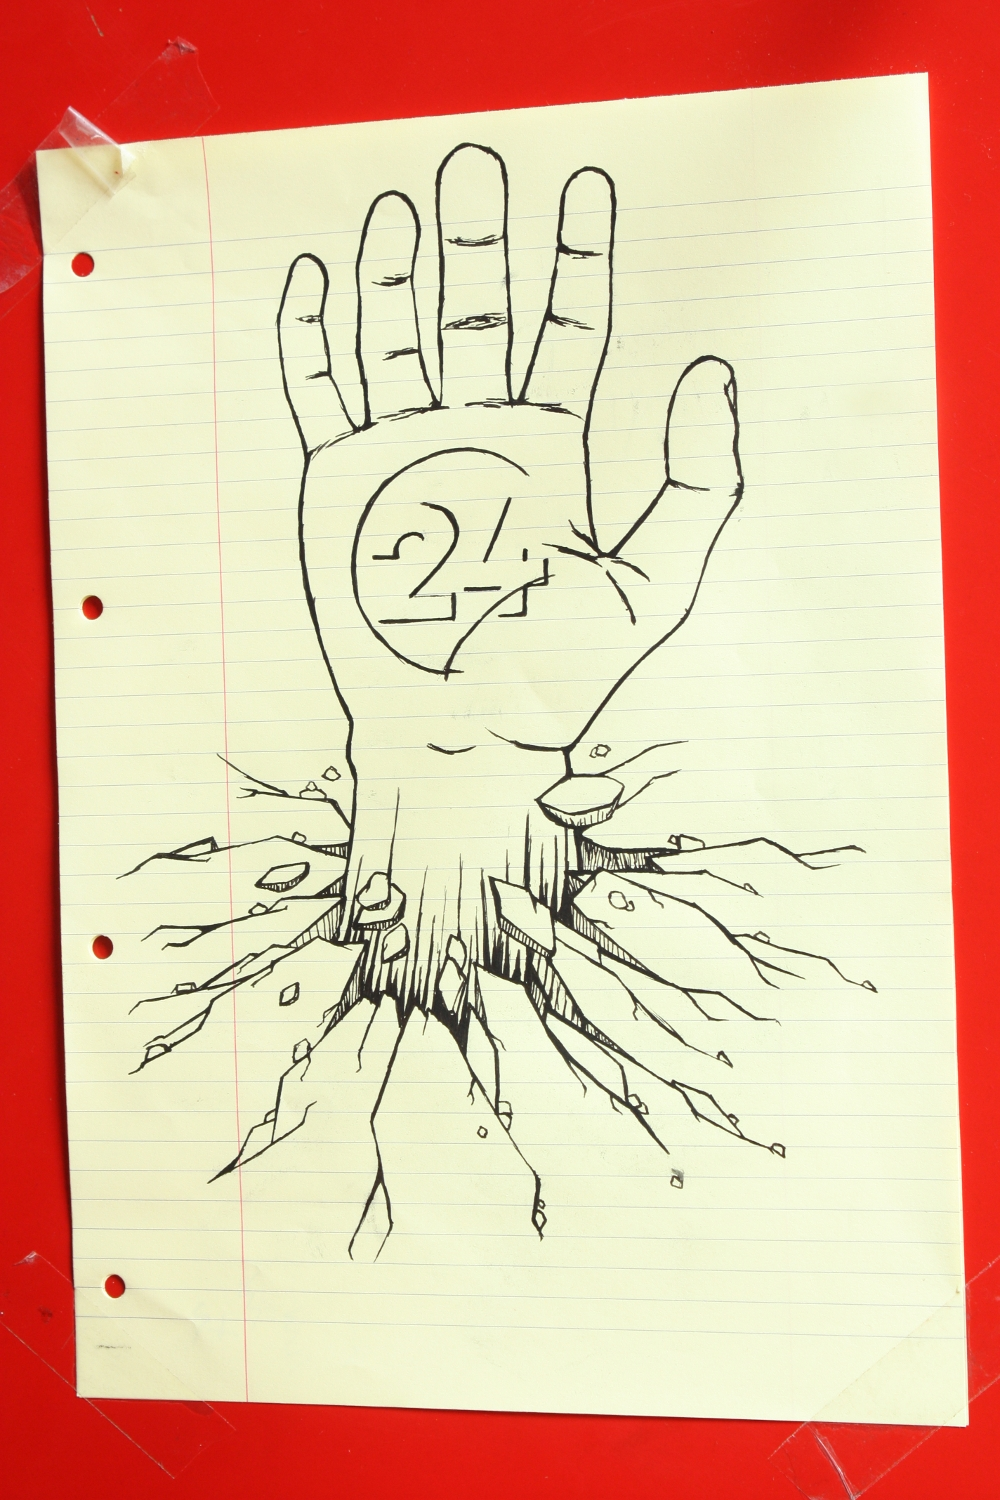
\includegraphics[width=0.24\textwidth]{img/IMG_5848.JPG}
                Une idée de visuel pour un T-Shirt vente
            \end{center}
            
            \begin{center}                     
                
\includegraphics[width=\textwidth]{img/splash24.png}
                Travail sur le logo de l'association, pour le thème \textit{tâches de peintures}
            \end{center}
                        
            \begin{center}
                
\includegraphics[width=\textwidth]{img/logo-TShirt-bichro.png}
                Proposition de visuel pour un T-Shirt vente
            \end{center}
                
            \begin{center}    
                \fbox{
\includegraphics[width=\textwidth]{img/affiche-soiree.png}}
                Proposition d'affiche concert  
            \end{center}
            
    \subsection{AEDI}
            
        \begin{center}
            %\fbox{
\includegraphics[width=0.3\textwidth]{img/WTFBBQjp.jpg}}
            \fbox{
\includegraphics[width=0.3\textwidth]{img/WTFBBQstorm.jpg}}
            \fbox{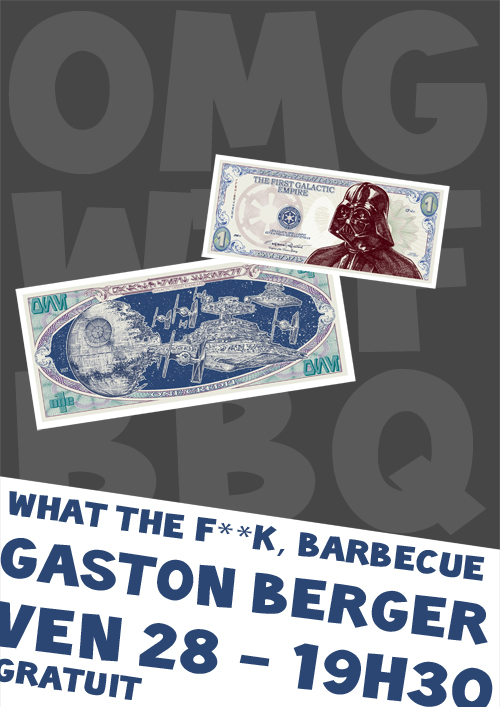
\includegraphics[width=0.3\textwidth]{img/WTFBBQsw.jpg}}
            %\fbox{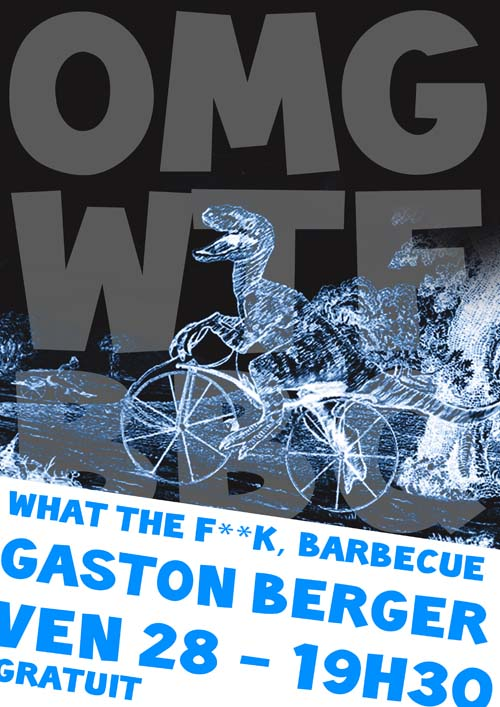
\includegraphics[width=0.3\textwidth]{img/WTFBBQvelo.jpg}}
            \fbox{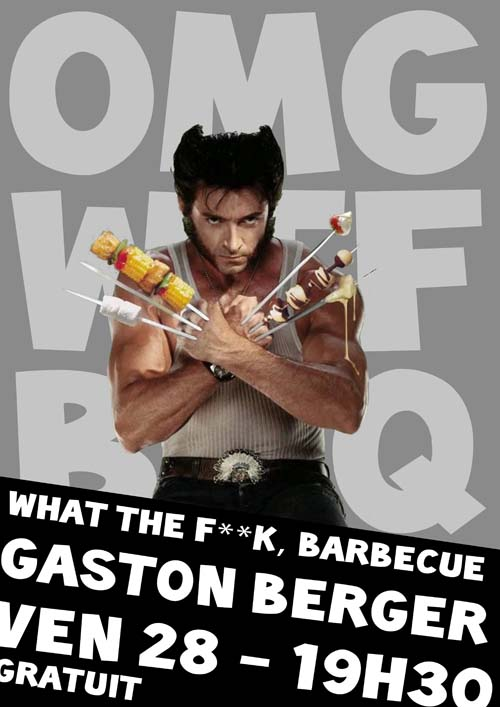
\includegraphics[width=0.3\textwidth]{img/WTFBBQwolv.jpg}}
            %\fbox{
\includegraphics[width=0.3\textwidth]{img/WTFBBQyoda.jpg}}
            Affiches pour le barbecue de fin d'année de l'AEDI
        \end{center}
        
        \begin{center}
            \centering
            
\includegraphics[width=0.9\textwidth]{img/yoda-or.jpg}\\
            Visuel de T-Shirt pour la promotion 52
        \end{center}




